\chapter{Synthesis in Example of a Magnetic Bearing on an Overhung Rotor}
Analysis and modeling techniques of the previous chapters will now be put to use in a practical example. The goal of which will be to reduce vibration on an overhung disk rotor system with the use of an Active Magnetic Bearing(AMB). An experimental test rig, not unlike the system used in the experimental example of \S\ref{ExperimentalPlots}, will be used to calibrate a  finite element theoretical model. Then, the theoretical model will be extended to include an AMB near the overhung disk. The model will be evaluated for stability, and parameters of the control algorithm for the AMB will be varied to attempt to eliminate the first natural frequency and stabilize the system.
\section{Physical System}
The rotor system of interest is depicted in Figure \ref{fig:OverhungDiagram}. Geometric parameters are listed in Table \ref{tab:GeometricParametersofOverhung}. The springs at nodes 1 \& 4 are intended to represent bushings, portion at node 6 is the rotating disk, and nodal numbers are shown as the rotor will be discretized for the finite element model.
\begin{figure}
	\centering
	\def\svgwidth{250pt}
	\import{figures/}{OverhungDiagram.pdf_tex}
	\caption{Overhung rotor system diagram.}
	\label{fig:OverhungDiagram}
\end{figure}
\begin{table}
	\centering
	\caption{Geometric parameters of the overhung rotor system.}
	\label{tab:GeometricParametersofOverhung}
	\begin{tabular}{cccccc}
		$ L[m] $&$ a[m] $&$ b[m] $&$ l_d[m] $&$ d_d[m] $&$ d_s[m] $\\\hline
		$ 0.5 $&$ 0.23 $&$ 0.13 $&$ 0.025 $&$ 0.075 $&$ 0.01 $
		\end{tabular}
\end{table}
\section{Experimental Results}
The rotor system was tested in a start-up from slow roll to $ 3000[RPM] $. Data shown here is taken from $ 1000[RPM] $ to $ 2000[RPM] $. A set of orthogonal eddy current sensors placed near the disk on the outboard side were used to measure the position of the shaft throughout the start-up. Position data was recorded at a sampling rate of $ 128000[Hz] $ with no processing applied. The resulting 3D orbit of the start-up is shown in Figure \ref{fig:MagExampleOrbit3D}. Of note is the necking in the 3D orbit that is indicative of high anisotropy inducing a negative whirl during the first natural frequency. Also resulting from the experiment is the full spectrum cascade plot of Figure \ref{fig:MagExampleCascade}, in which it is evident that synchronous vibration dominates the spectra. Though, for the production of the bode diagram (Figure \ref{fig:MagExampleBode}) there was a benefit in clarity from filtering the data to synchronous speed.
\begin{figure}
	\centering
	\includegraphics[width=.5\linewidth]{./figures/MagExampleOrbit3D.pdf}
	\caption{3D Orbit of the experimental overhung rotor system.}
	\label{fig:MagExampleOrbit3D}
\end{figure}
\begin{figure}
	\centering
	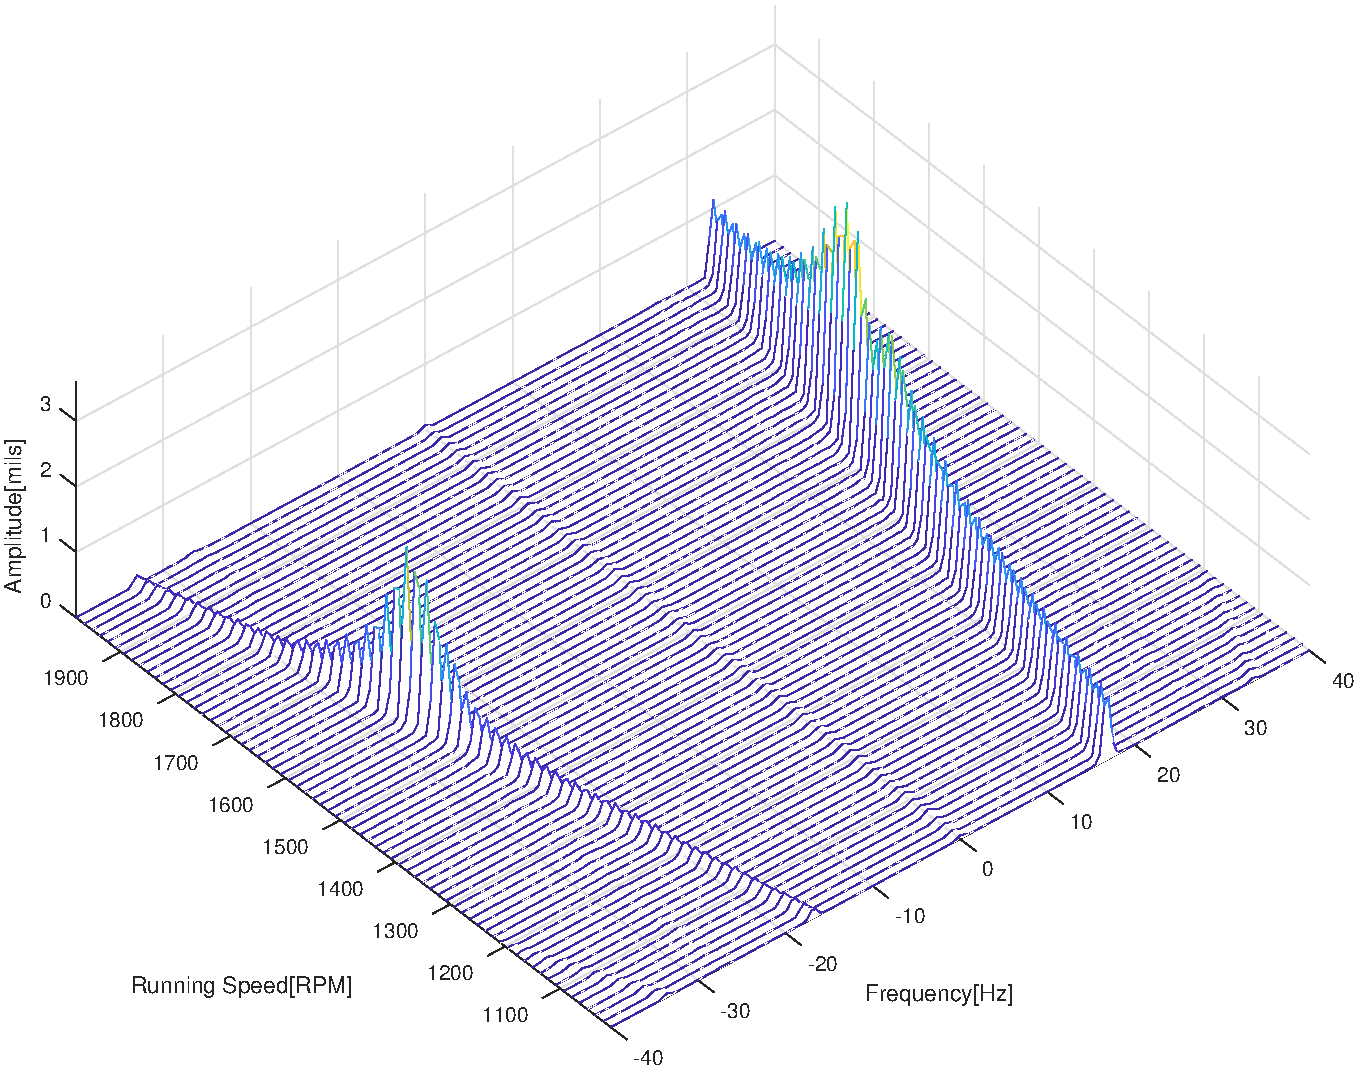
\includegraphics[width=.5\linewidth]{./figures/MagExampleCascade.pdf}
	\caption{Cascade of the experimental overhung rotor system.}
	\label{fig:MagExampleCascade}
\end{figure}
\begin{figure}[!htb]
	\def\width{.7\linewidth}
	\def\height{.4\linewidth}
	\def\sep{3em}
	\pgfplotsset{every picture/.style={trim axis left, trim axis right}, every axis/.style={ylabel style={xshift=0},xlabel style={yshift=0}}}%, every axis/.style={hide axis}}%
	\centering
	\import{figures/}{MagExampleBode.tex}
	\caption{Bode diagram of the experimental overhung rotor filtered to 1X.}
	\label{fig:MagExampleBode}
\end{figure}
\section{Theoretical Model}
To create a theoretical model for this rotor system. The shaft will be discretized into 7 elements a disk at node 6 and bearings at nodes 1 and 4, as depicted in Figure \ref{fig:OverhungDiagram}. In the experiment, a small length of shaft continued after the overhung disk and has been included in this model. The AMB will be included as a nodal point element with with stiffness and damping to be derived in \S\ref{Active Magnetic Bearing}. Parameter values for the finite element model are provided in Table \ref{tab:OverhungParameters}. Discovered values such as $ \eta_v $ and the stiffnesses of bearing are listed here, but the process for their determination is discussed.
\begin{table}
	\caption{Properties of disks, shaft elements, and bearings of the theoretical model.} \label{tab:MagTheoryRotorTable}
	\centering
	\label{tab:OverhungParameters}
	\begin{tabular}{rcccccc}
							&$\rho\left[\frac{kg}{m^3}\right]$	&$r[m]$					&$\nu$				&$E[Pa]$			&$ \eta_v[s] $	&$ \eta_h $	\\\hline
		\textbf{Shaft}		&$7850$					&$0.005$				&$0.3$				&$\num{210E9}$		&$ 0.0002 $		&$ 0 $		\\[-.2em]
							&$\rho\left[\frac{kg}{m^3}\right]$	&$r[m]$					&$l[m]$				&					&				&			\\\hline
		\textbf{Disks}		&$7850$					&$0.0375$				&$0.025$			&					&				&			\\[-.2em]
							&$k_y\left[\frac{N}{m}\right]$		&$k_z\left[\frac{N}{m}\right]$		&$c_y\left[\frac{Ns}{m}\right]$&$c_z\left[\frac{Ns}{m}\right]$&				&			\\\hline
		\textbf{Bearing A}	&$1.7\e{5}$				&$2.2\e{5}$				&$68$				&$88$				&				&			\\[-.5em]
		\textbf{Bearing B}	&$2.04\e{5}$			&$2.64\e{5}$			&$81.6$				&$105.6$			&				&			\\
	\end{tabular}
\end{table}
First the model is formed to match the experimental results. Known parameters, such as beam lengths, beam diameters, density of the material, and geometry of the disk and rotor are used to begin construction of the model. Then, guesses are made for the stiffnesses in the rotor bearings. The first natural frequency is calculated with the resulting model and its value compared to the experimentally found natural frequency from the bode diagram (fig.\ref{fig:MagExampleBode}). Stiffness are then adjusted to better match the natural frequency, and this is repeated until the natural frequency of the model matches the experiment. After this process, the stiffness was determined to be around $ 2\e{5} \left[\frac{N}{m}\right]$.\par
It is evident by inspection of the Bode diagram for the experimental system (fig.\ref{fig:MagExampleBode}), and the 3D orbit, that there is anisotropy in the system, leading to the dip in amplitude of one plane of vibration. It is also known from inspection of the frequency spectrum in the cascade of figure \ref{fig:MagExampleCascade} that in this speed range the orbit is in the opposite direction of the rotation--a phenomena only possible with anisotropy of the stiffness. Figures \ref{fig:HorVertStiffAniCompare}\&\ref{fig:PosNegStiffAniCompare} demonstrate this affect anisotropy has on both the real coordinates, as well as positive and negative whirl amplitudes. \par 
\begin{figure}
\begin{subfigure}{\textwidth/2}
	\centering
	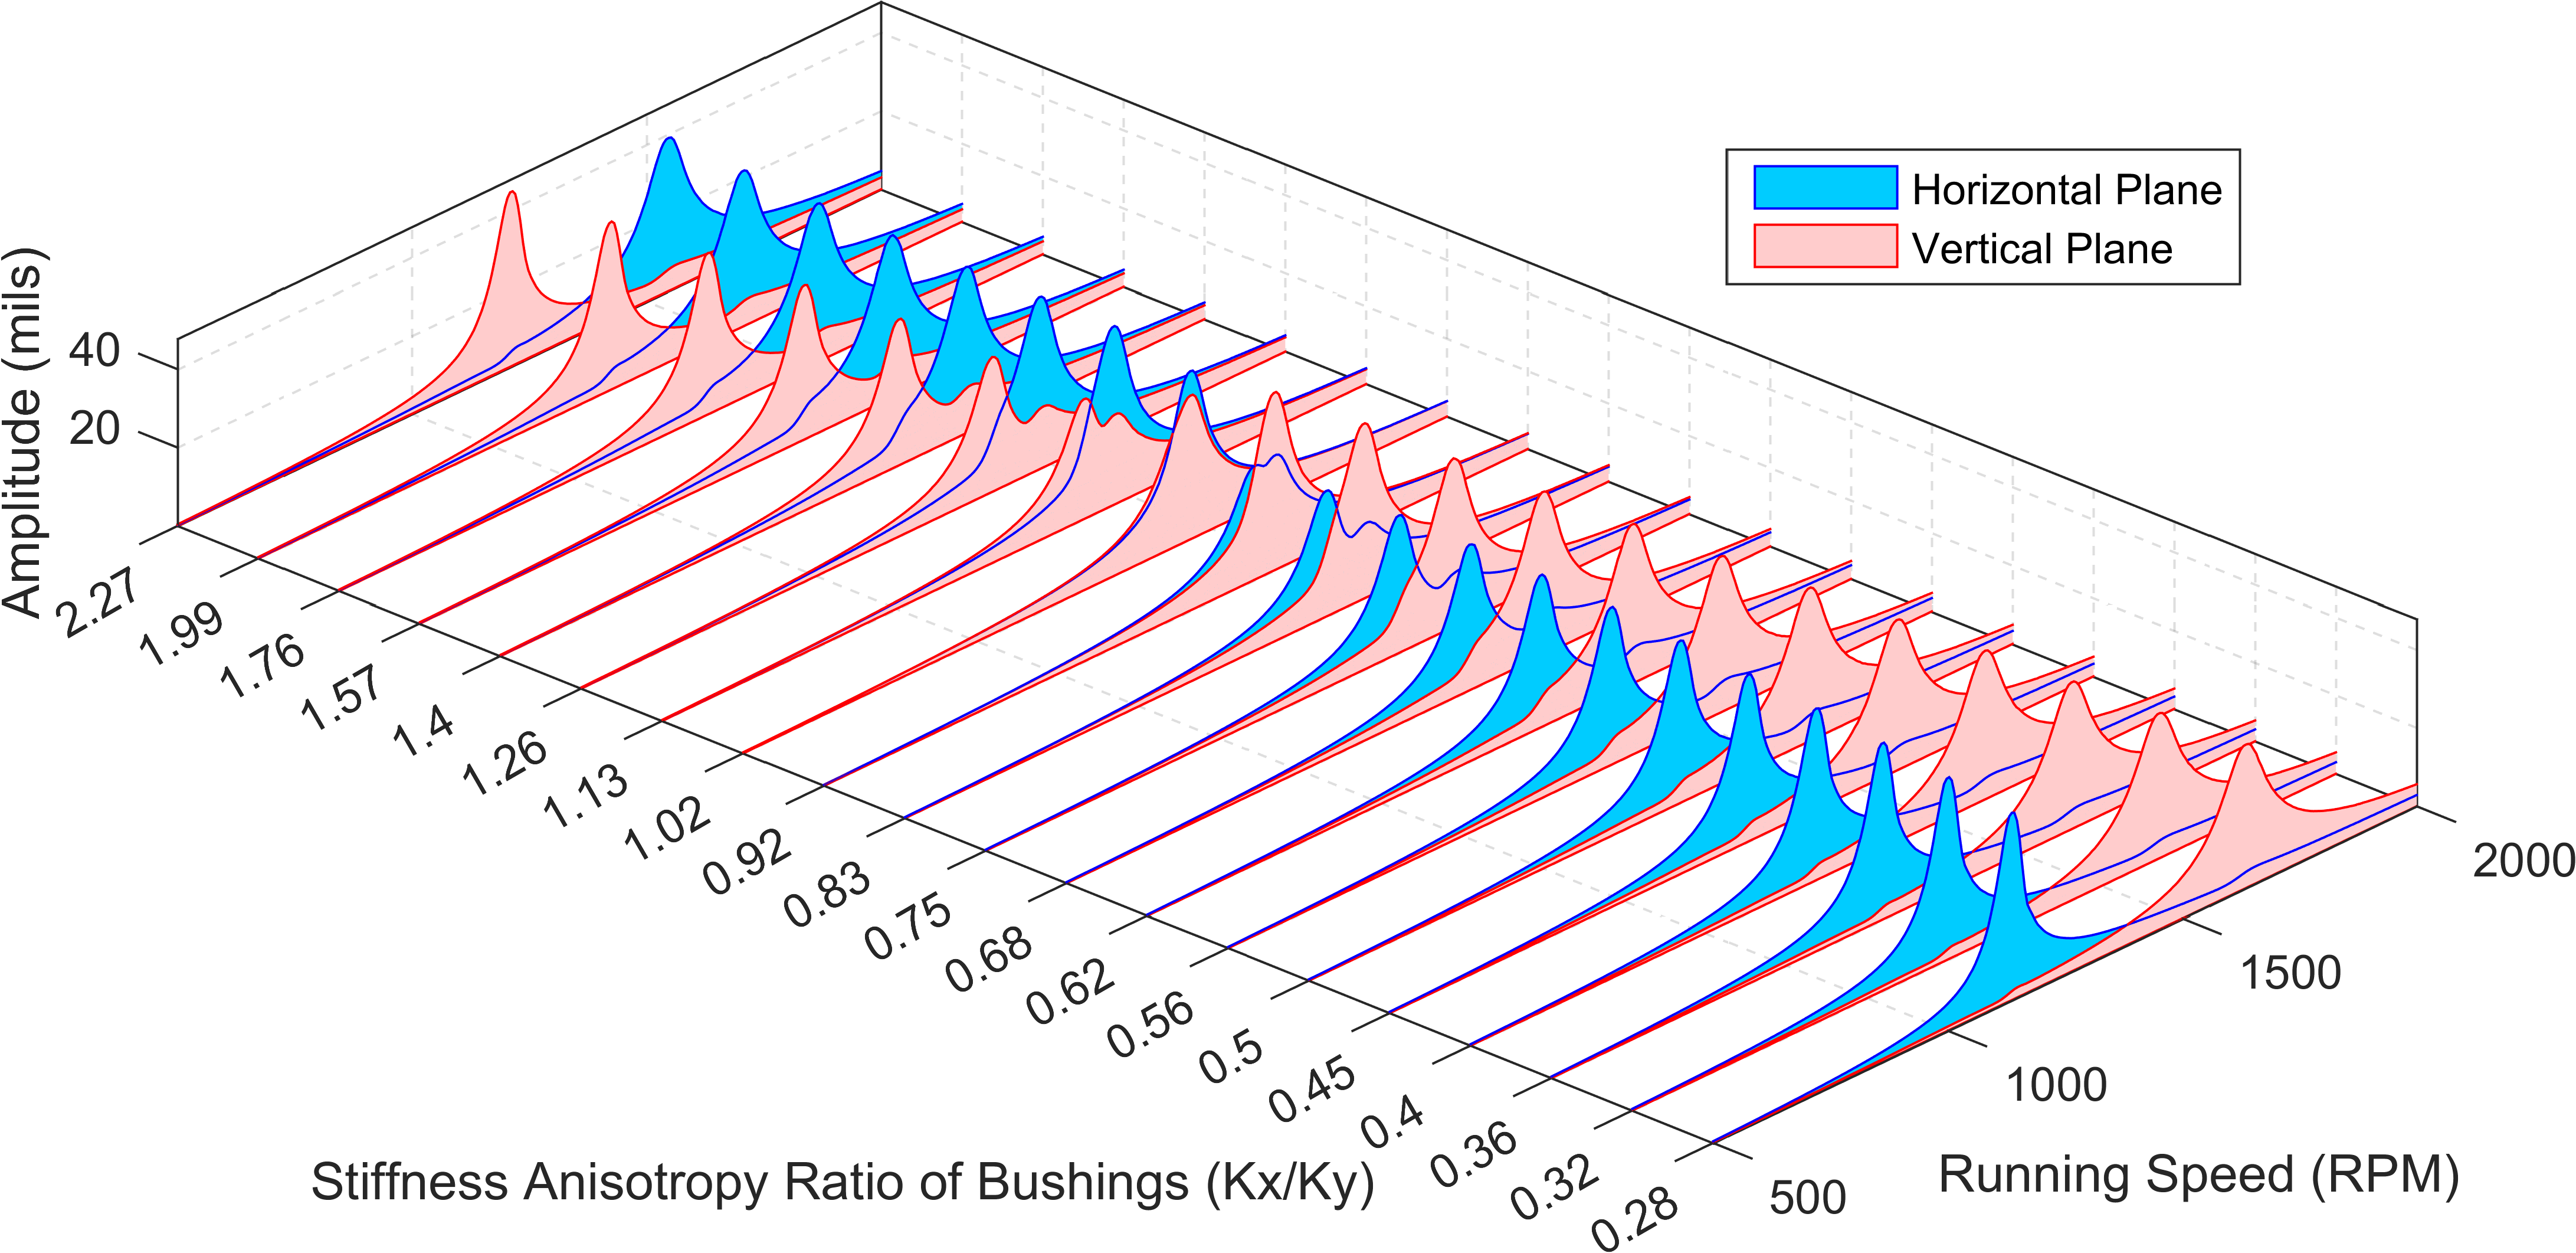
\includegraphics[width=\linewidth]{./figures/Images/Figure_6.png}
	\caption{3D Orbit of the experimental overhung rotor system.}
	\label{fig:HorVertStiffAniCompare}
\end{subfigure}
\begin{subfigure}{\textwidth/2}
	\centering
	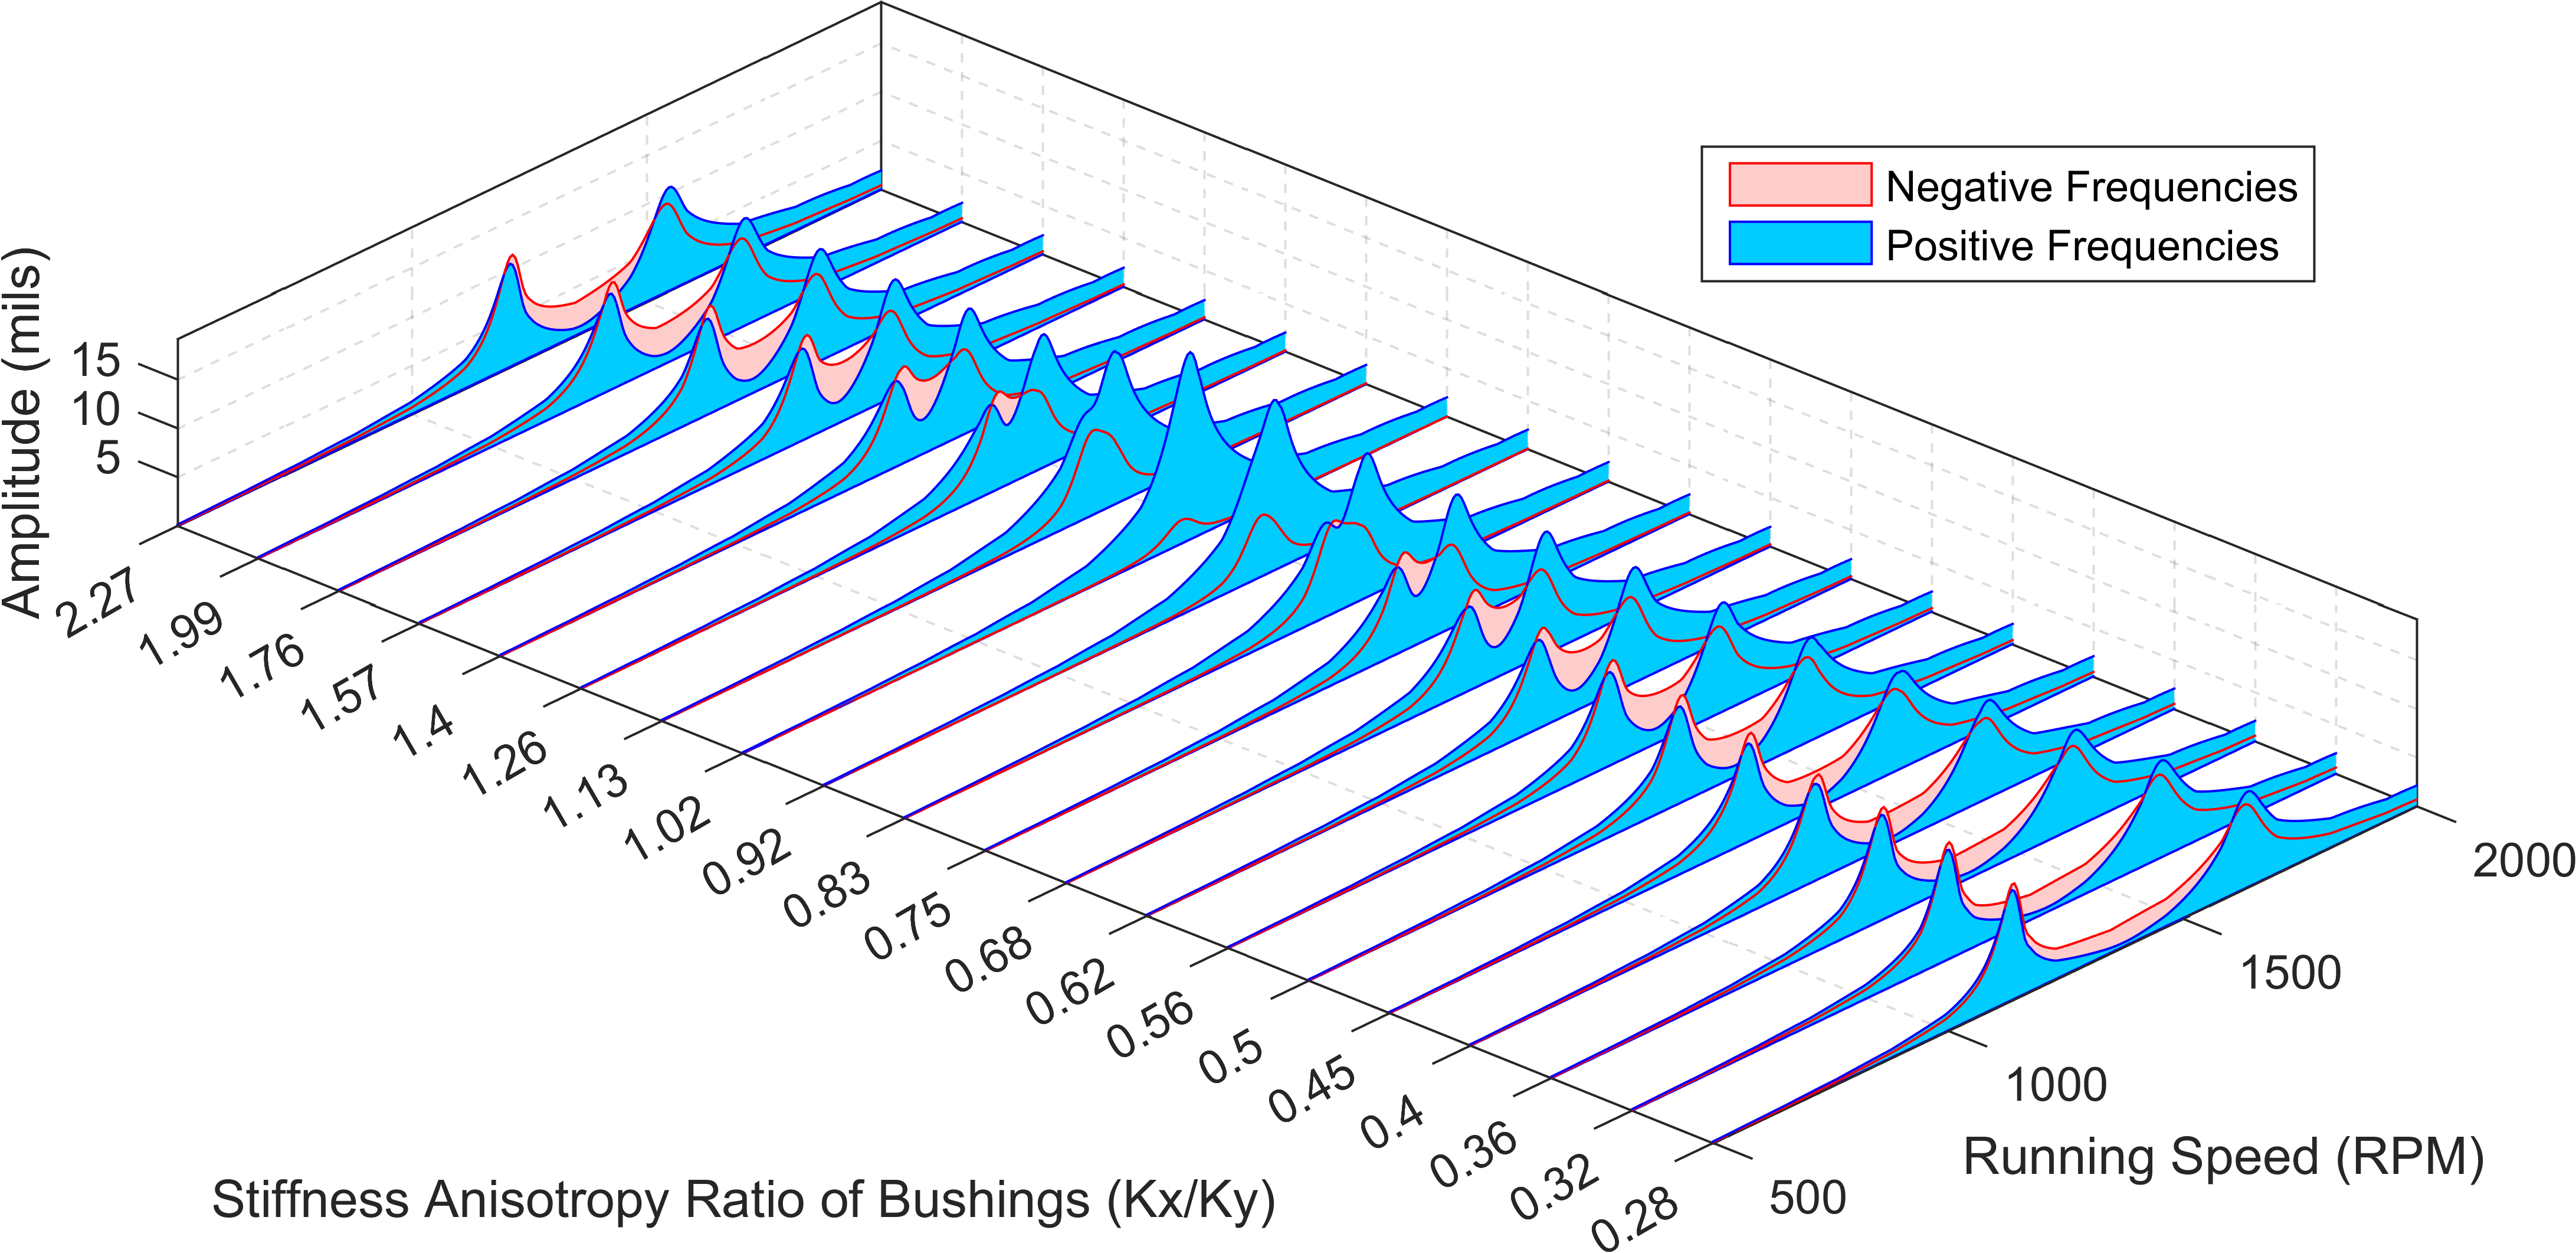
\includegraphics[width=\linewidth]{./figures/Images/Figure_5.png}
	\caption{3D Orbit of the experimental overhung rotor system.}
	\label{fig:PosNegStiffAniCompare}
\end{subfigure}
\end{figure}
Using the bode diagram, the stiffness anisotropy is adjusted until the shapes of the amplitudes and phases match the experimental results of figure \ref{fig:ExpExampleBode}. Then damping is added to the system to appropriately match the experimental results. The resulting bode diagram is Figure \ref{fig:MagTheoryBode}. Stiffnesses were determined to be $ k_y=1.7\e{5}[N/m]\ \&\ k_z=2.2\e{5}[N/m] $.
\begin{figure}[!htb]
	\def\width{.6\linewidth}
	\def\height{.4\linewidth}
	\def\sep{3em}
	\pgfplotsset{every picture/.style={trim axis left, trim axis right}, every axis/.style={ylabel style={yshift=.5em},xlabel style={yshift=0}}}%, every axis/.style={hide axis}}%
	\centering
	\import{figures/}{MagTheoryBode.tex}
	\caption{Damping ratio vs. spin speed with indication of threshold of stability.}
	\label{fig:MagTheoryBode}
\end{figure}
And now the resulting system is further described with an expanded speed range of $ 20000[RPM] $. The new Campbell diagram of Figure \ref{fig:MagTheoryCampbell}, the roots locus of Figure \ref{fig:MagTheoryRootLocus}. Additionally, the first three mode shapes are plotted for this theoretical model (Figures \ref{fig:MagTheoryShape1}, \ref{fig:MagTheoryShape2}, \& \ref{fig:MagTheoryShape3}). Note that the first mode is conical in shape, but the disk is far from an antinode at node 6 so it does not experience significant gyroscopic moments. This idea is supported by the campbell diagram, fig. \ref{fig:MagTheoryCampbell}, as the first mode natural frequency does not change significantly over the speed range. On the other hand, the second mode has its antinode atode 6 so the disk experience maximum gyroscopic moments and the second mode critical speed is much more dependent on speed.
\begin{figure}[!htb]
	\def\width{.6\linewidth}
	\def\height{.4\linewidth}
	\def\sep{3em}
	\pgfplotsset{every picture/.style={trim axis left, trim axis right}, every axis/.style={ylabel style={yshift=.5em},xlabel style={yshift=0}}}%, every axis/.style={hide axis}}%
	\centering
	\import{figures/}{MagTheoryCampbell.tex}
	\caption{Damping ratio vs. spin speed with indication of threshold of stability.}
	\label{fig:MagTheoryCampbell}
\end{figure}
\begin{figure}[!htb]
	\def\width{.6\linewidth}
	\def\height{.4\linewidth}
	\def\sep{3em}
	\pgfplotsset{every picture/.style={trim axis left, trim axis right}, every axis/.style={ylabel style={yshift=.5em},xlabel style={yshift=0}}}%, every axis/.style={hide axis}}%
	\centering
	\import{figures/}{MagTheoryRootLocus.tex}
	\caption{Damping ratio vs. spin speed with indication of threshold of stability.}
	\label{fig:MagTheoryRootLocus}
\end{figure}
\begin{figure}
	\def\cs{.29}
	\pgfplotsset{every picture/.style={trim axis left, trim axis right}, every axis/.style={yticklabel style={xshift=0,yshift=0},minor tick num=2}, grid style={line width=.1pt, draw=gray!20},major grid style={line width=.2pt,draw=gray!50},ticks=none,minor tick style={draw=none}}%, every axis/.style={hide axis}}% 
	\begin{subfigure}{\cs\textwidth}
		\centering
		\def\width{\linewidth}
		\def\height{\linewidth}
		\import{}{./figures/MagTheoryShape1.tex}
		\caption{Mode Shape 1.}
		\label{fig:MagTheoryShape1}
	\end{subfigure}
	\begin{subfigure}{\cs\textwidth}
		\centering
		\def\width{\linewidth}
		\def\height{\linewidth}
		\import{figures/}{MagTheoryShape2.tex}
		\caption{Mode Shape 2.}
		\label{fig:MagTheoryShape2}
	\end{subfigure}
	\begin{subfigure}{\cs\textwidth}
		\centering
		\def\width{\linewidth}
		\def\height{\linewidth}
		\import{figures/}{MagTheoryShape3.tex}
		\caption{Mode Shape 3.}
		\label{fig:MagTheoryShape3}
	\end{subfigure}
\end{figure}
\subsection{Active Magnetic Bearing}\label{Active Magnetic Bearing}
Magnetic pole-rotor relationship will be derived based on the detailed derivation in \cite{das2008vibration}. Assumptions made in this model are:
\begin{itemize}
	\item Air gap between the magnet pole face and the rotor is vanishingly small compared to the diameter of the shaft.\
	\item Flux leakage from the magnetic pole is negligible.
	\item Curvature of rotor surface under the pole face is ignored.
	\item A linear relationship of flux density and magnetic field is assumed.
	\item Hysteresis of the magnetic field is negligible.
\end{itemize}
These assumptions lead to a magnetic force due to coil current in the relationship of
\begin{equation}\label{key}
F_m=\frac{-k_mi^2}{l_g^2}
\end{equation}
where, $ k_m=\frac{\mu_0A_pN^2}{4} $, and $ \mu_0=4\pi\e{-7} $ is the absolute permeability in free air, $ N $ is the number of coil turns, $ A_p $ is the pole face area, $ i $ is the supplied electrical current, and $ l_g $ is the air gap.\par 
Consider a set of magnetic pole pairs in each the $ y\ \&\ z $ directions (i.e. One on the left and one on the right; one on top and one on bottom), where each pole pair has its own electrical circuit. There are 4 total magnets in this model, 2 in each direction, and 8 total poles where 2 form a magnet. All poles in the neutral position of the system will have a nominal air gap of $ g_0 $ and will be supplied by a bias current of $ i_0 $. Deviations of the current from this bias will be considered as $ i_y $ and $ i_z $. Deviations of the position from this neutral position are the displacements of the rotor at this beam axis location, $ v,\ \&\ w $. Therefore, total current will be $ (i_0\pm i_y)\ \&\ (i_0\pm i_z) $ for opposing poles in the $ y\ \&\ z $ directions respectively. Similarly, total gaps are given by $ (g_0\pm v)\ \&\ (g_0\pm w) $. Using these new definitions for the gap and current, and summing forces in the $ y\ \&\ z $ directions leads to the total forces
\begin{equation}\label{eq:MagneticForceNL}
F_y=K_m\left\{\left(\frac{i_0+i_y}{g_0+v}\right)^2-\left(\frac{i_0-i_y}{g_0-v}\right)^2\right\}\ \&\ F_z=K_m\left\{\left(\frac{i_0+i_z}{g_0+w}\right)^2-\left(\frac{i_0-i_z}{g_0-w}\right)^2\right\}
\end{equation}
where, $ K_m=k_m\cos(\alpha) $, and $ \alpha $ is half of the angle between the poles of a magnet. Linearizing the magnetic force equations \eqref{eq:MagneticForceNL}, while assuming the operating point for the system is where all positions and control currents are zero, results in
\begin{equation}\label{eq:MagneticForce}
F_y=k_ii_y+k_yv,\ \&\ F_z=k_ii_z+k_zw
\end{equation}
where, $ k_i=4K_m\frac{i_0}{g_0^2} $ is the current stiffness developed by the bias current, and $ k_y=k_z=k_s=-4K_m\frac{i_0^2}{g_0^3} $.
\subsubsection{Proportional Derivative Control}
A control algorithm is used to control the current sent to each pair of poles based on the position (proportional) and velocity (derivative) of the rotor. It is assumed that each set of pole pairs will receive opposite currents to act as a unit. Current control is given by 
\begin{equation}\label{eq:ControlCurrent}
i_y=-k_g(k_pv+k_v\dot{v}),\ \&\ i_z=-k_g(k_pw+k_v\dot{w})
\end{equation}
where, $ k_g $ is the power amplifier gain, $ k_p $ is the proportional gain, and $ k_v $ is the derivative gain. The total linearized force becomes
\begin{equation}\label{key}
F_y=-(k_gk_ik_p-k_s)v-k_gk_ik_v\dot{v},\ \&\ F_z=-(k_gk_ik_p-k_s)w-k_gk_ik_v\dot{w}
\end{equation}
so then the stiffness of the AMB is $ k_{mag}=(k_gk_ik_p-k_s) $ and the damping is $ d_{mag}=k_gk_ik_v $. As an equation of nodal stiffness and damping in the finite element system it can be represented by
\begin{equation}\label{eq:DiskNodeEquationofMotion}
\bunderline{\mathbf{D}}^m\dot{\vec{\mathbf{q}}}_k+\bunderline{\mathbf{K}}^m\vec{\mathbf{q}}_k=0
\end{equation}
where,
\begin{equation*}
\def\cs{2em}
\begin{array}{cc}
\bunderline{\mathbf{K}}^m=\left[\def\arraystretch{.8}\arraycolsep=0pt\begin{array}{cccccc}
\makebox[\cs]{$k_{mag}$}&\makebox[\cs]{0}&\makebox[\cs]{0}&\makebox[\cs]{0}&\makebox[\cs]{0}&\makebox[\cs]{0}\\
0&k_{mag}&0&0&0&0\\
0&0&0&0&0&0\\
0&0&0&0&0&0\\
0&0&0&0&0&0\\
0&0&0&0&0&0
\end{array}\right] & \bunderline{\mathbf{D}}^m=\left[\def\arraystretch{.8}\arraycolsep=0pt\begin{array}{cccccc}
\makebox[\cs]{$d_{mag}$}&\makebox[\cs]{0}&\makebox[\cs]{0}&\makebox[\cs]{0}&\makebox[\cs]{0}&\makebox[\cs]{0}\\
0&d_{mag}&0&0&0&0\\
0&0&0&0&0&0\\
0&0&0&0&0&0\\
0&0&0&0&0&0\\
0&0&0&0&0&0
\end{array}\right]
\end{array}
\end{equation*}
Knowing that the amplitude of vibration, $ A $, in the experimental system peaks at about 10 mils, or $ 2.54\e{-4}[m] $, the greatest possible velocity for synchronous vibration is determined using the simple equation $ v=(A/2)\omega $, where $ \omega $ is the whirl speed in rad/s. Under the assumption of synchronous vibration, $ \omega $ during the natural frequency is then $ 167.6[Rad/s] $. Leading to a velocity, $ v $, of $ 0.02[m/s] $. Looking also at the velocity in the upper speed range, knowing that the amplitude of vibration after the first natural frequency is equal to the eccentricity of the unbalance. With an eccentricity of $ 1\e{-5} $ and an upper speed of $ 15000[RPM] $, the velocity is calulated to be $ 0.008[m/s] $. Since the estimated velocity during the natural frequency is higher, it will be used to limit the output of the AMB controller. Since the total voltage supply of most digital to analog converters is limited to $ 10[V] $ the control voltage is calculated to be within this range for the given velocity and positions that will be seen under synchronous vibration. This results in a limitation of the term $ k_v $, which is proportional to the voltage control signal that is sent to the amplifier for conversion to control current. A value of $ 480[Vs/m] $ would max the converter, so the value to be determined must be less than this. With a similar, but separate, evaluation of the displacement leads to a cap of $ 500000[V/m] $ for $ k_p $--a value not anticipated to be necessary. The maximum force due to unbalance is $ \epsilon m_d\Omega^2 $, where $ \epsilon $ is the eccentricity, and $ m_d $ is the mass of the disk. At the maximum speed expected of $ 15000[RPM] $, the force will be $ 24[N] $. To counteract this force with a single coil would require $ 1.25[A] $, or $ 0.625[A] $ per coil in a opposing pair. The amplifier gain is assumed to be programmable to $ k_g=1[A/V] $, this leads to a reasonable choice of bias current at $ 0.5[A] $ to maintain a good resolution on the voltage output of the controller. The voltage should not need to peak above $ 1.25[V] $, and will rest at an output of $ 0.5[V] $. Now in the next section, control parameters $ k_v\ \&\ k_p $ will be determined to maximize stability of the system while also minimizing vibration.
\section{Addition of Magnetic Bearing to the Rotor Model}
In order to measure the effectiveness of the AMB, the Stability of the theoretical model before the addition is shown in Figure \ref{fig:MagTheoryStability}. The magnetic bearing added is modeled after a magnetic bearing that is currently in the lab at California Polytechnic State University. This theoretical exercise is intended to be followed by experimental verification not included in this work. The parameters used are listed in \ref{tab:MagBearingParameters} as well as the control values whose determinations will be evaluated.\par 
First the position of the AMB must be determined. By inspection of the mode shapes, it is evident that in the first mode (the mode we are most concerned about suppressing) a conical mode shape exists with increasing amplitude toward the end of the beam after the second bearing. It is also known that the source of vibration, the rotating disk, is located at nodal index 6. With both these pieces of information, node 7 is chosen as a starting point for the AMB for two reasons: having the AMB closer to the source of vibration reduces the phase lag between the source and the bearing, increasing the effectiveness of control; amplitude of vibration, according to the mode shape, is higher on the outboard side of the disk and placing the AMB on this side will minimize more vibration.\par 
 To determine best derivative control, the proportional control was set to zero and the derivative increased until the first mode on the Roots locus(fig. \ref{fig:MagTheoryRootLocus}) moved away from the imaginary axis, becoming more damped. The resulting movement of the Roots on the Roots Locus is given in Figure \ref{fig:MagTheoryRootLocusControllerTune}. Notice how none of the new modes that appear on the roots locus cross the real plane--this demonstrates the stability of the new system. Stability of the system with the AMB addition is confirmed in the stability plot of Figure \ref{fig:MagTheoryStabilityWith}. In fact from the roots locus with $ k_v=1 $ to the roots locus with $ k_v=10 $ the first mode of vibration is completely relegated to the imaginary axis and not reaching break-away for this entire speed range--this indicates that the first mode has been over-damped.\par 
 Proportional control, $ k_p $, was added after the ideal derivative control was determined, but it did not improve the performance of the controller. It is possible that the stiffness of the bearing inherent to the bias current is sufficient. In any case, proportional control in this scenario is only adding stiffness to the system, and with the objective being to minimize vibration, $ k_p $ does not help. So the optimal control is determined to be with $ k_v=10[Vs/m] $. The remaining parameters for this resulting controller are listed in table \ref{tab:MagBearingParameters}. It is worthwhile to note that this optimal control is standing on the basis that the feedback is of synchronous vibration only. In a scenario where there is significant sub or super-synchronous vibrations, this controller may exceed its voltage limit. It is recommended that the feedback signal be filtered to match rotor speed to ensure this scenario does not take place. Furthermore, without at least low-pass filtering of the feedback signal the control would certainly provide out of range signals due to the volatile nature of derivatives of discrete signals.\par 
 The frequency spectrum is provided showing the result of the AMB application in the bode diagram of Figure \ref{fig:MagTheoryBodeCompare}. Certainly it can be concluded that the AMB is successfully performing the desired task of reducing the vibration while also inproving the stability of the system.\par 
 Now the result from this synthesis exercise can be implemented on the actual experimental test rig with the AMB set to the control parameters suggested. The power of the finite element method in this application is the ability to move components around with ease. For instance, with the changing of just two parmeters in the input file for this model, a new simulation is create for complete levitation of the overhung rotor. The AMB is put in place of bearing b and the resulting frequency spectrum is plotted in Figure \ref{fig:MagLevTheoryBodeCompare}
\begin{table}
	\centering
	\caption{Active Magnetic Bearing Parameters.}
	\begin{tabular}{cccccccc}
		$\alpha[rad]$&$g_0[m]$&$i_0[A]$&$k_p[\frac{V}{m}]$&$k_v[\frac{Vs}{m}]$&$k_g[\frac{A}{V}]$&$ N[\#]$&$A_p[m^2]$\\\hline
		$\frac{\pi}{8}$&$2.5\e{-3}$&$0.5$&$0$&$10$&$1$&$800$&$\frac{5}{100*100}$
	\end{tabular}
	\label{tab:MagBearingParameters}
\end{table}
\begin{figure}
	\begin{subfigure}{\textwidth/2}
		\def\width{.8\linewidth}
		\def\height{.4\linewidth}
		\pgfplotsset{every picture/.style={trim axis left, trim axis right}, every axis/.style={ylabel style={yshift=-20},xlabel style={yshift=35}},every x tick scale label/.style={at={(xticklabel* cs:1,.3cm)},anchor=near xticklabel}}%, every axis/.style={hide axis}}%
		\centering
		\import{figures/}{MagTheoryStability.tex}
		\caption{Stability plot of rotor without AMB, threshold of stability:$ \ 4646[RPM] $.}
		\label{fig:MagTheoryStability}
	\end{subfigure}
	\begin{subfigure}{\textwidth/2}
		\def\width{.8\linewidth}
		\def\height{.35\linewidth}
		\pgfplotsset{every picture/.style={trim axis left, trim axis right}, every axis/.style={xlabel style={yshift=-2em},xlabel style={yshift=25,at={(axis description cs:0.5,1.05)},anchor=north}},every x tick scale label/.style={at={(xticklabel* cs:1,.3cm)},anchor=near xticklabel}}%, every axis/.style={hide axis}}%
		\centering
		\import{figures/}{MagTheoryStabilityWith.tex}
		\caption{Stability plot of rotor with AMB, indicates complete stability through speed range.}
		\label{fig:MagTheoryStabilityWith}
	\end{subfigure}
\end{figure}
\begin{figure}[!htb]
	\def\width{.7\linewidth}
	\def\height{.5\linewidth}
	\def\sep{3em}
	%\pgfplotsset{every picture/.style={trim axis left, trim axis right}}%, every axis/.style={ylabel style={yshift=0em},xlabel style={yshift=0}}}%, every axis/.style={hide axis}}%
	\centering
	\import{figures/}{MagTheoryRootLocusControllerTune.tex}
	\caption{Roots locus of Overhung rotor system with varying $ k_v $.}
	\label{fig:MagTheoryRootLocusControllerTune}
\end{figure}
\begin{figure}[!htb]
	\def\width{.6\linewidth}
	\def\height{.4\linewidth}
	\def\sep{3em}
	\pgfplotsset{every picture/.style={trim axis left, trim axis right}}%, every axis/.style={ylabel style={yshift=0em},xlabel style={yshift=0}}}%, every axis/.style={hide axis}}%
	\centering
	\import{figures/}{MagTheoryBodeCompare.tex}
	\caption{Bode diagram at node 6 comparing the rotor without AMB(solid) and with AMB(dashed).}
	\label{fig:MagTheoryBodeCompare}
\end{figure}
\begin{figure}[!htb]
	\def\width{.6\linewidth}
	\def\height{.4\linewidth}
	\def\sep{3em}
	\pgfplotsset{every picture/.style={trim axis left, trim axis right}}%, every axis/.style={ylabel style={yshift=0em},xlabel style={yshift=0}}}%, every axis/.style={hide axis}}%
	\centering
	\import{figures/}{MagLevTheoryBodeCompare.tex}
	\caption{Bode diagram at node 6 comparing the rotor without AMB(solid) and with AMB(dashed) for complete levitation at node 4.}
	\label{fig:MagLevTheoryBodeCompare}
\end{figure}